\documentclass[a4paper,12pt,numbers=noenddot]{report}

\usepackage{polski}
\usepackage[utf8]{inputenc}
\usepackage{graphicx}
\usepackage{cite}
\usepackage{float}
\usepackage{url} 
\usepackage{hyperref}
\usepackage{amsmath}
\usepackage{gensymb}
\usepackage{pdfpages}
\usepackage[nottoc,numbib]{tocbibind}
\usepackage{etoolbox}
\usepackage{enumitem}

\usepackage{titlesec, blindtext, color}

\titleformat{\chapter}[hang]{\Huge\bfseries}{\thechapter{. }}{0pt}{\Huge\bfseries}


\usepackage[
  inner = 3cm,
  outer = 2.5cm,
  top = 2.5cm,
  bottom = 2.5cm,
]{geometry}


\title{TYTUŁ pracy}
\date{\today}
\author{Hubert Marcinkowski}

\begin{document}
	\nocite{*}
	\pagenumbering{gobble}
	%\maketitle
	
\includepdf{first_page.pdf}

	\newpage
	\pagenumbering{arabic}
	\tableofcontents
	\newpage
	%\setcitestyle{square}	
	
\chapter{Wstęp}
Projektowanie interfejsów jest tematyką bardzo złożoną i nadzwyczaj kluczową w procesie tworzenia aplikacji, w tym, między innymi, gier komputerowych. Złe zaprojektowanie tej części w prosty sposób może przyczynić się do całkowitego braku zrozumienia całego przesłania gry przez użytkowników. Istnieje wiele metodologii mających na celu analizę jakości stworzonego projektu - od metod całkowicie subiektywnych po takie, które stawiają za zadanie sprowadzenie jak największej części elementów do postaci parametrycznej. 

- Trudne zadanie związane z tym, że poszukiwany jest pewien zbiór reguł, który ułatwiłby proces projektowania. 
- Część z przedstawianych rozwiązań wybitnie nie pasuje do dziedziny mobilek
- Problemy związane z projektowaniem dla mobilek
- Przygotowane zostały heurystyki, które mają na celu dokładne określenie jakie warunki aplikacja musi spełniać, by mogła zostać dobrze odebrana przez użytkowników
- coś o tym, że użytkownik w czasie gry często zostaje postawiony przed przyswojeniem bardzo abstrakcyjnego zadania w celu zrozumienia, a co za tym idzie grania w daną grę

W pracy tej opisane zostało badanie mające na celu zweryfikowanie wpływ spełniania tych heurystyk na pozna

\chapter{Cel, założenia oraz zakres pracy}
Celem tej pracy było zbadanie wpływu określonych heurystyk tworzenia interfejsów na jakość przyswajania nowych mechanik gry mobilnej. Zbadane zostały wybrane dwie opisane przez H. Desuvire oraz Ch. Wiberg \cite{ArticlePLAY} reguły, które odnoszą się do użyteczności projektowanych aplikacji.

!
Zwykle heurystyki dla gier mobilnych sprawdzają grywalność, tutaj wykorzystane zostają, by sprawdzić ich wpływ na jakość przyswojenia nowych reguł przedstawianych użytkownikowi, mechanik rozgrywki.
!

! TUTAJ TE HEURYSTYKI TRZEBA WRZUCIĆ

Przeprowadzone zostało doświadczenie, które miało na celu określenie, czy gra, której interfejs spełnia zadane warunki jest lepiej rozumiana i szybciej opanowywana od takiej, której nie są spełnione wybrane heurystyki. Przygotowana została w tym celu aplikacja na urządzenia mobilne, w której użytkownikom postawione zostają zadania, które nie wpisują się w popularne szablony obecnych gier na te platformy. Wyróżnione zostały cztery różne wersje interfejsów przedstawianych użytkownikowi, każda wersja spełniała inny złożenie heurystyk.

\chapter{Grywalność w grach mobilnych}

\section{Mechanika gry}
Przed rozpoczęciem analizy, kluczowym zdaje się określenie, co dokładnie definiowane jest pojęciem mechaniki gry komputerowej. 
\section{Grywalność}
 .... definiuje pojęcie grywalności jako ...

\section{Kontrola}
Kontrolą określane jest...

\chapter{Znane metody badawcze}

\section{Heurystyki PLAY}

\section{Inne heurystyki}

\chapter{Badanie przyswajania mechanik gry}
Sprawdzenie poziomu, w jakim użytkownik zrozumiał mechaniki w grze w którą gra, nie należy do prostych zadań. Na początku wymagane jest odpowiednie sprecyzowanie założeń jakie muszą być spełnione do przeprowadzenia badań. Równie ważnym aspektem jest przygotowanie aplikacji, która jest w stanie zapewnić sprawdzenie podstawowych danych z przebiegu rozgrywki. Następnie należy zaprojektować odpowiednie badanie, które pozwoli na zebranie wyników, które pozwolą na określenie parametrów przebiegów gry.
\section{Założenia}
Gdy użytkownik po raz pierwszy styka się z pewnym rozwiązaniem, którego nigdy wcześniej nie widział w żadnej innej grze, to przed faktycznym zaczęciem rozgrywki musi on najpierw zrozumieć zadaną mu mechanikę. Założyć można zatem, iż to jak dany gracz radzi sobie na tym etapie gry jest ściśle skorelowane z tym jak dobrze rozumie postawione przed nim zadanie. Zbierając odpowiednie dane można zatem wydobyć informację o tym, jaki poziom przystosowania do rozgrywki osiągnął gracz. Przygotowując różne wersje gry spełniające w innym stopniu wybrane heurystyki PLAY będzie zatem możliwe ocenić która z nich zawiera w sobie mechaniki, których gracze musieli spędzić najmniej czasu na nauce.

%\section{Zastosowany sprzęt}
%Do przebiegu eksperymentu zastosowanych zostało trzy rózne 
\section{Gra mobilna}
Na potrzeby badań wykorzystana została mobilna gra \textit{Sphaze}, która należy do gatunku aplikacji logicznych. Przed użytkownikiem stawiane jest abstrakcyjne zadanie doprowadzenia obracających się kul do środka labiryntu składającego się z współcentrycznych pierścieni. Sfery poruszają się jedynie po wyraźnie zarysowanych ścieżkach. Wygląd przykładowego poziomu zawierającego dwie kule oraz trzy pierścienie zamieszczony został na rysunku \ref{fig:sphaze_1}.

\begin{figure}[h!]
	\centering
  	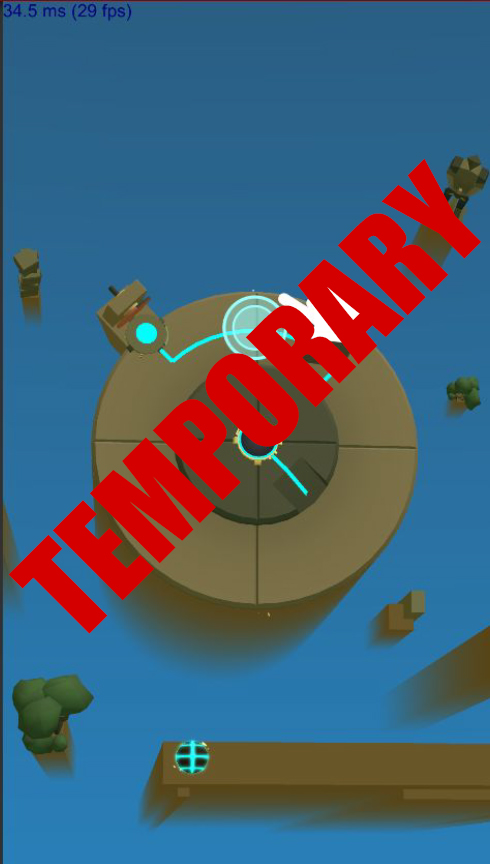
\includegraphics[height=8cm]{fig/tmp.jpg}
	\caption{Wygląd przykładowego poziomu gry \textit{Sphaze}.}
	\label{fig:sphaze_1}
\end{figure}

Osoba grająca nie ma wpływu na ruch sfer, jedynie na obrót pierścieni planszy. Każda rotacja na tych elementach powoduje zmianę połączeń między ścieżkami na nich się znajdującymi. Kule cały czas poruszają się do przodu, chyba że spotkają na swojej drodze skrzyżowanie. Wybierają wtedy ścieżkę, którą zdefiniować można jako "najbardziej prawą". Oznacza to, mając możliwość skręcenia w prawo, zawsze wybiorą tą opcję. Gdy nie ma możliwości obrotu w prawo, sprawdzane jest, czy dostępna jest ścieżka na wprost. W następnej kolejności przeprowadzony zostaje test, czy istnieje skręt w lewo. W przypadku braku możliwości wyboru żadnej z przedstawionych opcji, uznawane jest, że natrafiono na "ślepy zaułek", konieczne jest zatem zawrócenie.

Użytkownik decyduje również, z którego miejsca na planszy ma wystartować jaka sfera. Wprowadzenie pierwszej kuli na strefę labiryntu traktowane jest jako rozpoczęcie rozgrywki. Przykładowe punkty startowe, na których ustawić można kule ukazane zostały na rysunku \ref{fig:sphaze_startpoints_1}. Zauważyć można, iż znajdują się one wszystkie na obrzeżach planszy. Jest to reguła, którą gracz jest w stanie bardzo szybko zauważyć. Dzięki temu na późniejszych poziomach gracze nie próbują ich szukać w żadnym innym miejscu. Z racji na fakt, iż "rozbijają" one okrągłą sylwetkę planszy wyjątkowo łatwo je dostrzec nawet gdy gra aktualnie ich nie wyróżnia. 
Na każdym poziomie zdefiniowane jest ograniczenie czasowe, którego przekroczenie jednoznacznie wiąże się z koniecznością powtórzenia zadanej planszy. Czasomierz, którego zadaniem jest informowanie użytkownika o tym jak dobrze sobie on radzi, rozpoczyna odliczanie wraz z rozpoczęciem rozgrywki, czyli gdy pierwsza kula zacznie poruszać się w przestrzeni poziomu. 

\begin{figure}[h!]
	\centering
  	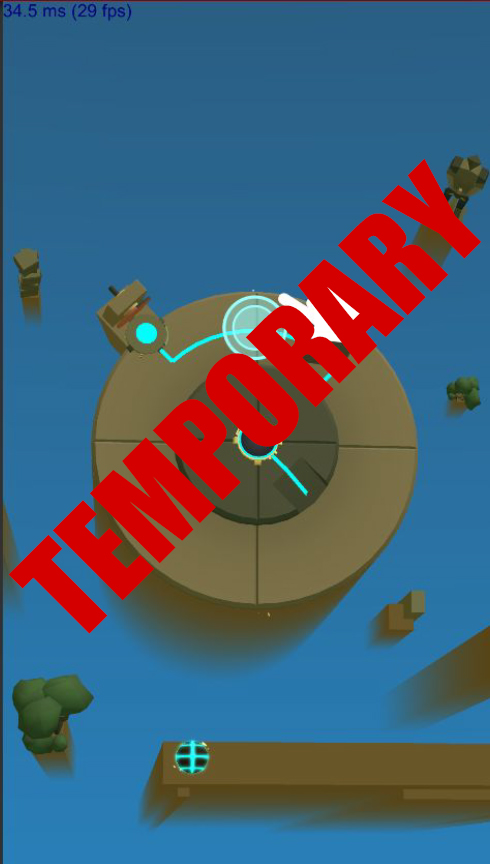
\includegraphics[height=8cm]{fig/tmp.jpg}
	\caption{Przykładowe rozmieszczenie punktów startowych na poziomie. Punkty startowe zostały oznaczone czerwonymi okręgami.}
	\label{fig:sphaze_startpoints_1}
\end{figure}

Gracz ma ograniczoną kontrolę nad rozgrywką, gdyż jego akcje wpływają jedynie pośrednio na jej przebieg. Obrót pierścieni wpływa jednie na możliwości ruchu, jakimi dysponują kule. Zadaniem użytkownika jest dostosowanie się do tego stanu i przewidzenie, jak obiekty poruszać się będą w zadanym przez niego środowisku. Nieświadome podejmowanie decyzji może bowiem prowadzić do sytuacji, które szybko potrafią stać się mało zrozumiałe dla użytkownika, który nie do końca rozumie, co się dzieje w przestrzeni gry.

	\subsection{Samouczki}
Wymagane jest zatem, by gracz przyswoił podstawowe prawa tej gry jak najszybciej. W przeciwnym wypadku spodziewać się można, iż prędko zacznie odczuwać frustrację spowodowaną pozornie małym wpływem jego akcji na finalny wynik gry. 

Z tego też powodu przygotowane zostały tzw. samouczki mające na celu wyjaśnienie użytkownikowi kluczowych mechanik. Nowe informacje przekazywane są stopniowo. Każdy kolejny element kluczowy jest najpierw przedstawiany w prostym, kontrolowanym środowisku, a następnie powtarzany już w coraz bardziej złożonych sytuacjach. 
W przeprowadzanym badaniu analizowane były trzy główne mechaniki: 
\begin{itemize}
\item sposób na startowanie rozgrywki na danym poziomie, 
\item obracanie pierścieniami,
\item ruch kulek (fakt, iż zawsze skręcają one w najbardziej prawą ścieżkę.
\end{itemize}

W celu poprawnego nauczenia tych mechanik przygotowane zostały dwa testowe poziomy. W pierwszym z nich przedstawiane są podstawowe dwie zasady gry. Akcja jaką, użytkownik ma wykonać zostaje przedstawiona wizualnie bez użycia tekstu. Sam gracz musi zrozumieć, że jego ruchem powinno być odzwierciedlenie tego, co pokazywane mu jest na ekranie. Należy zauważyć, że użytkownik nie zawsze jest w stanie również przewidzieć co się wydarzy, gdy wykona zadane mu zadanie. Dopiero po wykonaniu ukazanej akcji jest w stanie przeanalizować jaki wpływ miały jego ruchy na przestrzeń gry.
Wygląd poszczególnych etapów tego poziomu dla jednej wersji gry przedstawiony został na rysunku \ref{fig:tut_L1_1}.

\begin{figure}[h!]
	\centering
  	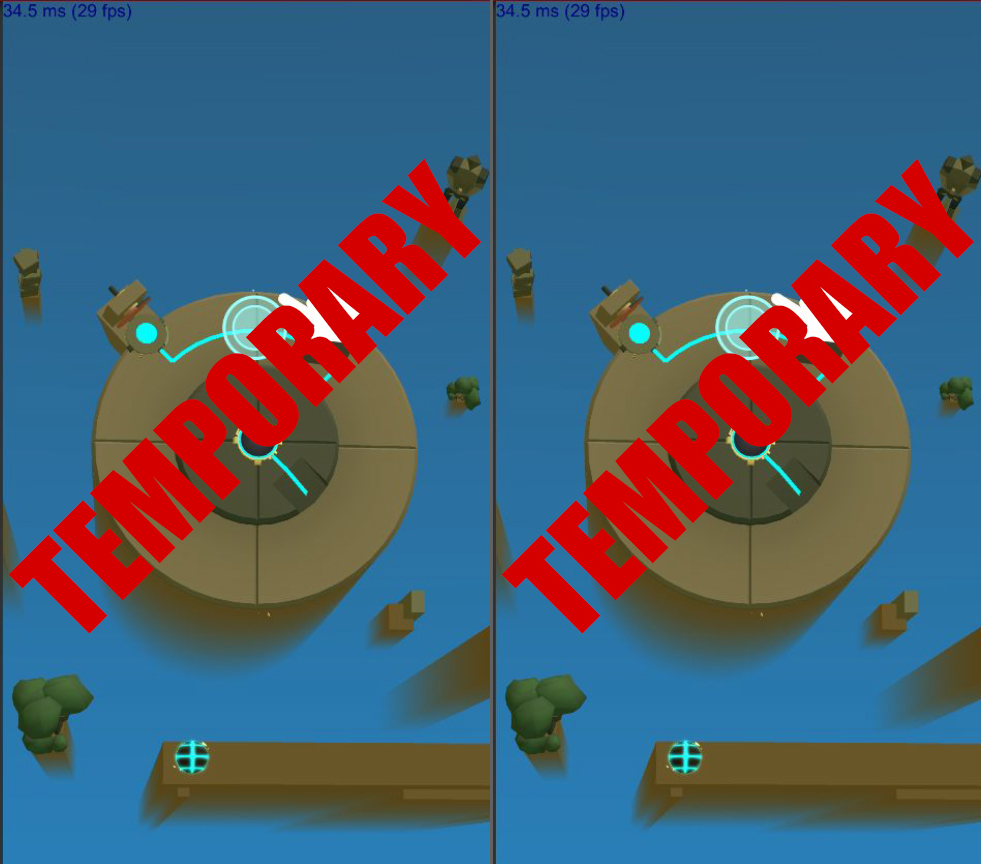
\includegraphics[height=8cm]{fig/tmp2.jpg}
	\caption{Wygląd pierwszego samouczka przed którym postawiony jest gracz.}
	\label{fig:tut_L1_1}
\end{figure}

Plansza dla tego poziomu składa się z dwóch poziomu składa się z dwóch pierścieni. Nie można poruszać pierścieniem w samym środku, co sprawia, że jedynym fragmentem labiryntu, z którym użytkownik może wchodzić w interakcję jest zewnętrzny pierścień.
Gdy gracz włączy ten poziom wymagane jest od niego aby najpierw obrócił właśnie ten element. Celem jest doprowadzenie do połączenia ścieżek znajdujących się na pierścieniach. Gdy gracz wykona ruch powodujący rozłączenie tych dróg, samouczek powróci do tego etapu. Pozwala to w łatwy sposób uzmysłowić użytkownikowi, o wadze, jaką ma stworzenie odpowiedniej drogi dla kul. 
Następnym zadaniem jest ustawienie jedynej sfery na poziomie w jej miejscu startowym. Samouczek znika dopiero w momencie poprawnego wykonania tej akcji. Gdy to nastąpi i użytkownik nie wprowadzi dalszych zmian w obrocie pierścieni, kula w szybki sposób dociera do środka labiryntu, a co za tym idzie - kończy poziom.

Drugi samouczek ustawiony został dopiero na trzeciej planszy. W tym miejscu chcemy zwrócić uwagę gracza na zachowanie kul w momencie dotarcia do skrzyżowania. Wygląd tego poziomu zobaczyć można na rysunku \ref{fig:tut_L3_1}. Labirynt w tym wypadku składa się z trzech pierścieni, z czego z dwoma z nich użytkownik może wejść w interakcję. Obecny tutaj samouczek wyzwala się dopiero w momencie, gdy za przeprowadzonymi wcześniej akcjami gracza sfera dotrze do skrzyżowania znajdującego się na środkowym pierścieniu. Zostaje wtedy zabrana użytkownikowi kontrola a kamera skupia się na problematycznym miejscu. Oprócz tego, zanim zostanie wykonany manewr kulki, zostaje pod nią narysowana strzałka wskazująca, w którą stronę ona skręci. Gry kulka opuszcza skrzyżowanie, kamera wraca do podstawowej pozycji a ruchy gracza znowu wpływają na układ pierścieni. Całość opisanych akcji zajmuje podczas normalnej gry tylko ułamek sekundy, dlatego czas gry zostaje w tym momencie czterokrotnie spowolniony. 
\begin{figure}[h!]
	\centering
  	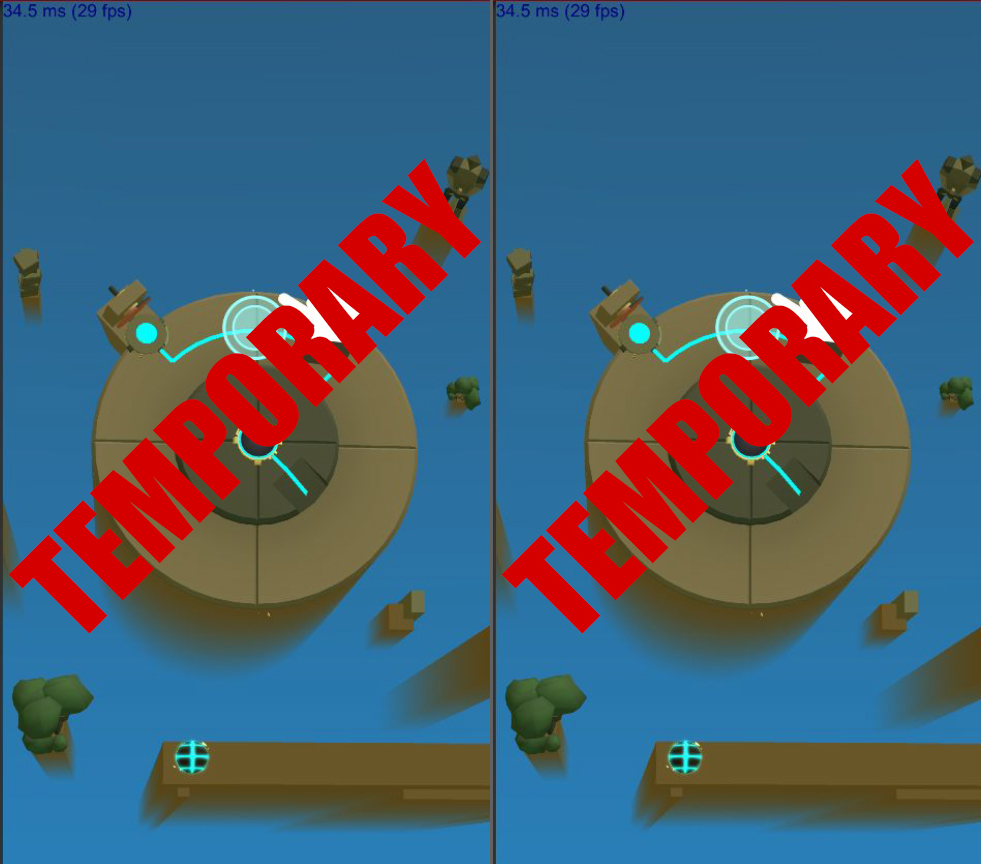
\includegraphics[height=8cm]{fig/tmp2.jpg}
	\caption{Wygląd poziomu zawierającego samouczek tyczący się skrętu kul. Czerwonym okręgiem zaznaczone zostało skrzyżowanie.}
	\label{fig:tut_L3_1}
\end{figure}
Mimo tego, całość przedstawionych operacji trwa niecałe trzy sekundy. Oprócz tego składa się z ruchów kamery, które użytkownik widzi jedyny raz w tym miejscu rozgrywki. Istnieje zatem szansa, iż nie uda mu się zrozumieć pełnego przekazu, który miał być zawarty w tym samouczku. Dlatego też następne dwa poziomy, które zobaczyć można na rysunku \ref{fig:tut_L3_2}, stworzone zostały z myślą o tym, by pomóc graczom ze zrozumieniem mechaniki skrętu kul. W obydwu tych poziomach rozwiązanie, które jest początkowo sugerowane, powoduje powstanie sytuacji, w której kulka skręcając w prawo oddala się od środka labiryntu. Użytkownicy, którzy nie rozumieją jeszcze sposobu poruszania się kulki bardzo szybko są wtedy w stanie zauważyć, że kryje się za tym jakiś algorytm. Gdy to zostanie osiągnięte, zrozumienie w jaki sposób wyznaczana jest trasa dla sfery przychodzi znacznie łatwiej.

\begin{figure}[h!]
	\centering
  	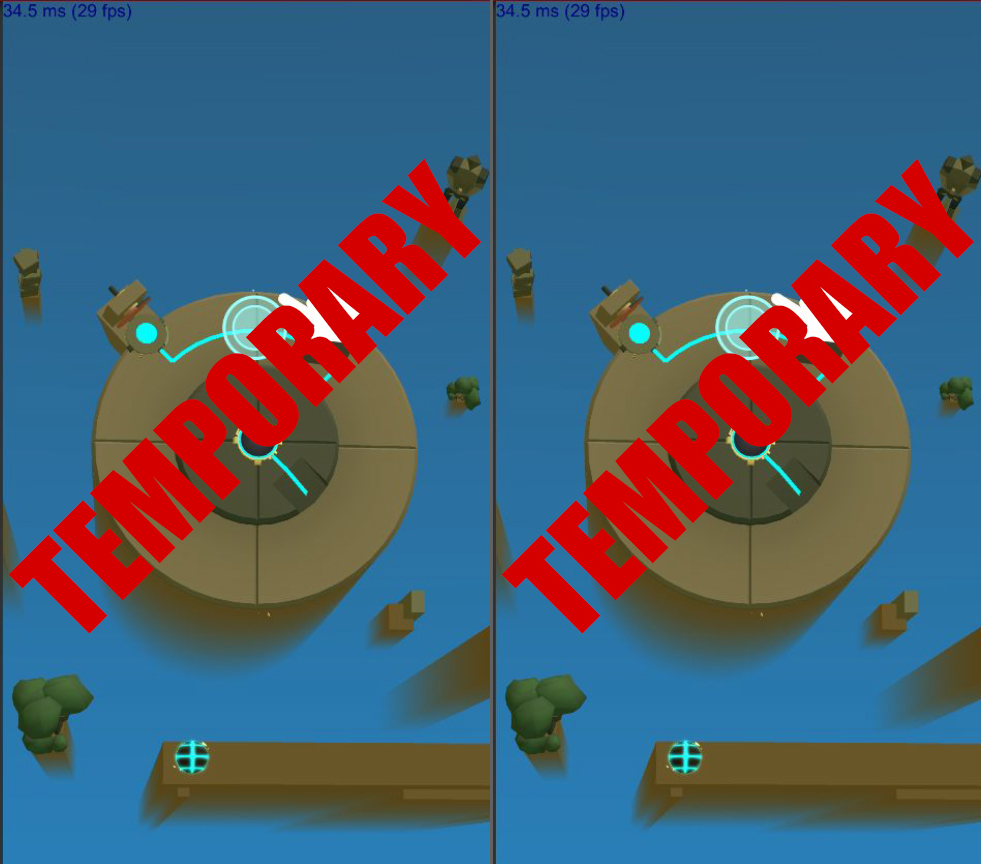
\includegraphics[height=8cm]{fig/tmp2.jpg}
	\caption{Początkowy wygląd czwartego i piątego poziomu gry \textit{Sphaze}. Mają one na celu pomóc użytkownikowi zrozumieć mechanikę ruchu kul.}
	\label{fig:tut_L3_2}
\end{figure}

\section{Heurystyki}
Z listy heurystyk PLAY \cite{ArticlePLAY} wybrane zostały dwie zaliczające się do kategorii użyteczności oraz mechanik gry. Określają one, jak projektowana powinna być gra, by grywalność była jak największa. Wyróżnione heurystyki zostały wybrane jako nietrywialne i subiektywnie najprostsze do efektywnego zweryfikowania. Opisane one zostały w tabeli \ref{tab:tab1}.

\begin{table}[h!]
  \centering
  \caption{Wybrane analizowane heurystyki PLAY z dziedziny informacji o statusie i wyniku.}
  \label{tab:tab1}
  \begin{tabular}{|r|l|}
    \hline
    1. & Wskaźniki wyniku są płynne, oczywiste, dostępne oraz nie wpływają na rozgrywkę.\\
    \hline
    2. & Sterowanie jest intuicyjne i mapowane w sposób naturalny.\\
    \hline
  \end{tabular}
\end{table}

\section{Rodzaje interfejsów}
W rozgrywce widoczny jest jedynie jeden wskaźnik statusu - określa on pozostały użytkownikowi czas na poziomie. Przedstawić go można jako jako dwuwymiarowy przycisk podobny do tego, który używany jest do zatrzymania gry, lub jako siatkę w przestrzeni gry. Każde podejście ma swoje zalety. W przypadku elementu 2D użytkownik nie ma wątpliwości co do jego informacyjnego przeznaczenia. Dla wersji w świecie gry nie zawsze to musi być spełnione. Wręcz przeciwnie, użytkownik, który dopiero uczy się na czym polegają mechaniki gry może odczuć frustrację bądź zniechęcenie wywołane tym, że nie jest możliwe wejście w interakcję z elementem umieszczonym w bezpośredniej przestrzeni gry. Plusem tego rozwiązania jest dużo bardziej zrozumiałe połączenie między fragmentami rozgrywki. Prostszym zdaje się zrozumienie powodu startowania czasomierza w chwili ustawienia pierwszej kulki na planszy, gdy zarówno labirynt, jak i reprezentacja zegara współdzielą ze sobą jedną przestrzeń.

Spełnianie drugiej z wybranych heurystyk określić można jako sterowanie zbliżone do tego, jak wyglądałoby wykonywanie akcji z gry w normalnym świecie. Tak więc, aby obrócić pierścień naturalnym zdaje się ruch przeciągania. Również przeniesienie kulki z miejsca na miejsce wydaje się oczywiste, że powinno zostać wykonane poprzez "złapanie" jej i przeciągnięcie w miejsce docelowe gdzie finalnie następuje jej "upuszczenie". Dzięki takiemu podejściu do tych mechanik uzyskane zostaje wrażenie fizyczności obiektów w przestrzeni gry. Stworzona zostaje iluzja, że zachodzi faktyczna interakcja z obiektami, które wyświetlane są na ekranie. Inaczej prezentuje się to przy mniej realnej wersji interakcji. Wykorzystana w niej zostaje inna znana mechanika z urządzeń mobilnych - proste kliknięcie w interesujące nas miejsce. Tym sposobem użytkownik jest w stanie zakomunikować, w którą stronę chce obrócić pierścień poprzez dotknięcie go z odpowiedniej strony. Przeniesienie kulki w tym scenariuszu odbywa się poprzez dotknięcie wybranej sfery, a następnie powtórzenie tej akcji dla miejsca docelowego. W tym wypadku użytkownik, który dobrze rozumie te mechaniki może znacznie szybciej wykonywać akcje w trakcie gry. Wiąże się to jednak z utratą części wiarygodności, którą uzyskać można było sposobem pierwszym.

Na podstawie wybranych heurystyk przygotowane zostały zatem cztery wersje gry. Każda z nich spełnia inną kombinację zadanych założeń. Takie podejście pozwala na dokładne przetestowanie, jaki wpływ zasady te mają na grywalność aplikacji. 
\subsection{Interfejs SWIPE 2D}
Jako pierwszy wyróżniony został interfejs \textit{SWIPE 2D}, który w założeniu spełnia zarówno pierwszą, jak i drugą heurystykę. Jego reprezentację graficzną dla pierwszego poziomu gry zobaczyć można na rysunku \ref{fig:interface_swipe_2d}. Zegar zdefiniowany jest w nim jako element dwuwymiarowy znajdujący się w górnej części ekranu, a wszelkie interakcje rozwiązane są poprzez jak najwierniejsze odwzorowanie ich odpowiedników z rzeczywistości. Spodziewać się zatem można najmniejszej ilości błędów popełnianych przez użytkowników już od samego początku gry. Również różnice w czasach pojedynczego testu powinny być dla tej wersji względnie niewielkie.
\begin{figure}[h!]
	\centering
  	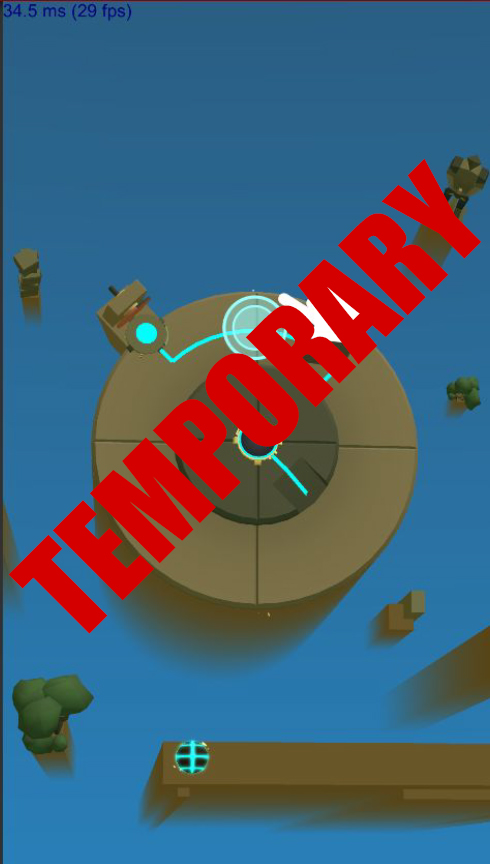
\includegraphics[height=8cm]{fig/tmp.jpg}
	\caption{Wygląd poziomu pierwszego dla wersji gry wykorzystującej interfejs \textit{SWIPE 2D}.}
	\label{fig:interface_swipe_2d}
\end{figure}
\subsection{Interfejs SWIPE 3D}
Wersja interfejsu wykorzystująca mechanikę przesuwania lecz niespełniająca pierwszej z wybranych heurystyk określona została mianem \textit{SWIPE 3D}. Jego wygląd zaprezentowany jest na rysunku \ref{fig:interface_swipe_3d}. Siatka stanowiąca zegar umieszczona została w świecie gry, jako element znajdujący się wizualnie przy wyborze kul. Położenie to zostało zmienione z racji na charakterystyczne ustawienie kamery w grze. Nie pozwala ono na ustawienie tak ciężkiego elementu powyżej labiryntu, gdyż wpływałoby to negatywnie na estetykę gry. To rozwiązanie wpływać może rozgrywkę, gdyż niewykluczona jest sytuacja, w której gracz może odbierać czasomierz jako element, z którym  należy wejść w jakąś interakcję. Spodziewać się tu można zatem większej ilości błędów, które popełniane mogą być przy pierwszej styczności użytkownika z grą.
\begin{figure}[h!]
	\centering
  	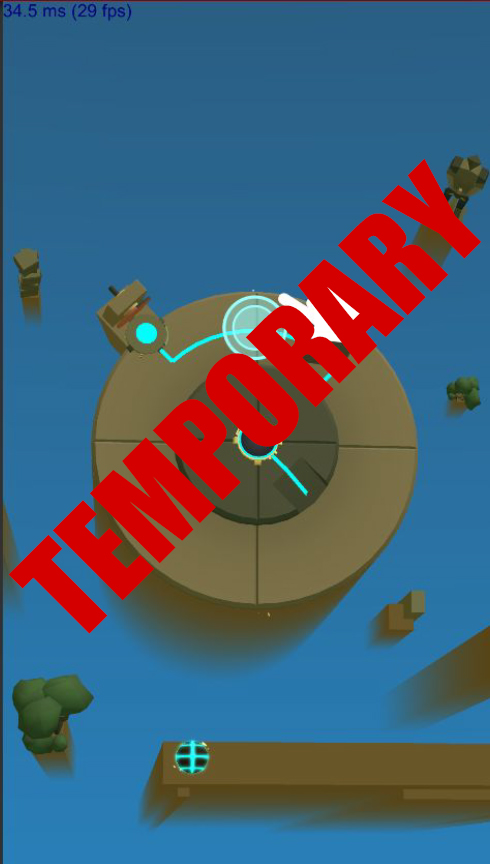
\includegraphics[height=8cm]{fig/tmp.jpg}
	\caption{Wygląd poziomu pierwszego dla wersji gry wykorzystującej interfejs \textit{SWIPE 3D}.}
	\label{fig:interface_swipe_3d}
\end{figure}
\subsection{Interfejs CLICK 2D}
Interfejs \textit{CLICK 2D} wizualnie nie rózni się od wersji \textit{SWIPE 2D}. Zmieniony jest tu jednak styl sterowania głównymi mechanikami gry na takie, które są w znacznie mniejszym stopniu reprezentacją rzeczywistych interakcji. Cechują się one tym, że by osiągnąć ten sam cel wykonywane mogą być znacznie szybsze ruchy (kliknięcie zamiast przesuwania palca po ekranie). Oznaczać to może, że doświadczony użytkownik jest w stanie uzyskać w tej wersji lepsze czasy niż ten, który umiejętnie posługuje się wersją z mechaniką przesuwania. Idąc tym tropem założyć można, iż różnica w czasach przechodzenia poszczególnych poziomów będzie zatem tutaj zauważalnie większa, gdyż wymaga on nauczenia się mniej intuicyjnej zasady gry.
\subsection{Interfejs CLICK 3D}
Podobnie jak w poprzednim przypadku, w wersji interfejsu \textit{CLICK 2D} brak jest różnic wizualnych względem \textit{SWIPE 2D}. W tym wypadku jednak nie jest spełniona żadna ze sprawdzanych heurystyk. Oznaczać to może, że wyniki dla tego wypadku będą najmniej korzystne. Spodziewać się można dużej ilości początkowych błędów spowodowanych mniej odciętym od całości gry zegarem oraz większych różnic w statystykach podczas przechodzenia tego samego poziomu dwukrotnie przez pojedynczego gracza.
\section{Struktura badania}
Na potrzeby przeprowadzenia testów przygotowane zostało badanie mające na celu wydobycie z przebiegów gry przydatnych informacji. 
Użytkownik miał za zadanie zagrać w przygotowaną wcześniej grę w ściśle określony sposób:
\begin{itemize}
\item przejść pierwszych pięć poziomów,
\item zagrać w arbitralnie dobraną liczbę następnych plansz (przynajmniej 5),
\item ponownie rozegrać pierwszych pięć poziomów.
\end{itemize}
Zarówno przed jak i po przeprowadzeniu badania osoba testująca nie musiała wypełniać żadnej ankiety odnośnie swoich wrażeń z gry. Oznacza to też, iż dane takie jak płeć, czy wiek gracza nie były brane pod uwagę w dalszej ocenie wyników. Gra automatycznie zapisywała wyniki badania do pliku, który później podlegał analizie.

Zauważyć należy iż dane zbierane były tylko dla pierwszych pięciu plansz. Powtórzenie ich przejścia na koniec indywidualnego testu jest kluczowe dla wyników badań. Przy pierwszym podejściu do poziomów 1-5 gracz nie wie, czego aplikacja może od niego wymagać. Jest to jego pierwsze starcie z mechanikami, których musi się nauczyć. \
Inaczej sprawa się ma z drugimi wynikami danej osoby badanej. Z racji tego, że wymagane jest by przeszła ona przynajmniej 10 poziomów, założyć można, iż zaznajomiła się ona z podstawowymi prawami gry. Różnice pomiędzy tymi wynikami pozwalają na określenie jak dużego postępu dokonał gracz, o ile lepiej zrozumiał zadane mechaniki. Zminimalizowana zostaje w ten sposób różnica pomiędzy umiejętnościami różnych osób. Gdy porównywane są one do samych siebie nie nie trzeba brać pod uwagę czynników, takich jak przykładowo predyspozycje do sprawnego przechodzenia gier logicznych.

Pomijalny staje się również wpływ, jaki miało środowisko, w którym przeprowadzany był eksperyment. W uproszczeniu założyć można, że w warunkach, jakie były zapewnione użytkownikom zarówno oświetlenie, jak i poziom hałasu utrzymywał się na jednym poziomie dla jednego testu.

Same testy odbywały się zarówno na wyciszonym, względnie odizolowanym pomieszczeniu ale także w dużo trudniejszych warunkach - jako część większych wydarzeń, bądź podczas jazdy komunikacją miejską. 

Do celów badania przygotowane zostały cztery wersje gry, które zawierały w sobie opisane wcześniej interfejsy. Osobie badanej przyznawana była losowo wybrana aplikacja z tej puli i przedstawiana była jako jedyna wersja gry. 
Badane były osoby, które nigdy wcześniej nie spotkały się z grą będącą obiektem testów. Miały one za zadanie przejść zadane poziomy bez żadnej wcześniejszej informacji o tym, jaki jest chociażby warunek przejścia do następnej planszy. Informacja o tym, że wyniki podlegają zapisowi przekazywana była dopiero wtedy, gdy wymagane było, by osoba testowana przystąpiła ponownie do pierwszych pięciu poziomów. Miało to na celu możliwe zminimalizowanie presji czasu, która mogłaby się pojawić przy otrzymaniu aplikacji do testowania.(JAKIŚ LINK?)

Dla każdego przejścia poziomu przez danego użytkownika zebrane zostały następujące dane:
\begin{itemize}
\item czas absolutny, 
\item czas ruchu kuli,
\item ilość obrotów pierścieni,
\item ilość dotknięć ekranu.
\end{itemize}
Oprócz tego, obliczona została dodatkowa zmienna, która zależna jest od czasu absolutnego oraz czasu ruchu kuli - czas myślenia użytkownika.

	\subsection{Czas absolutny}
Czas, który użytkownik potrzebował na przejście poziomu, licząc od jego załadowania określany jest mianem absolutnego $t_{abs}$. Zawiera on w sobie długość trwania obejrzanej przez użytkownika animacji wejścia poziomu, a jego liczenie przerywane jest wraz z wejściem ostatniej kuli na poziomie do środka labiryntu. Czas ten nie zawiera zatem w sobie informacji o tym, jak długo użytkownik pozostawał na ekranie podsumowującym dany poziom. Spowodowane to było obserwacją, że czas spędzony w tym ekranie uznany został za pomijalny w przeprowadzanych badaniach.
	\subsection{Czas kuli}
Oprócz obliczania tego, ile czasu potrzebne było użytkownikowi na przejście poziomu wymiernym okazało się również sprawdzanie jak optymalne ścieżki wybrane zostały dla sfer. Wszystkie plansze, które wykorzystane zostały w badaniu korzystały tylko z jednej kulki, która na każdej z nich poruszała się z tą samą szybkością. Oznacza to, że droga ta jest wprost proporcjonalna do czasu, w jakim poruszała się kulka - $t_{ball}$. Jego obliczanie zaczyna się wraz z wykonaniem przez użytkownika akcji startu sfery w wybranym punkcie startowym labiryntu, a kończy się, podobnie jak w przypadku $t_{abs}$, wraz z dotarciem tej sfery do środka. Im większa ta zmienna, tym bardziej można przypuszczać, iż użytkownik nie przewidział, jak zachowa się kula na planszy. Zaobserwować można tutaj, w zależności od urządzenia na którym przeprowadzone zostały pomiary, iż zmienna ta jest obciążona błędem pomiaru rzędu $5 ms$.
	\subsection{Czas myślenia}
Przydatnym w celach analizy wyników okazał się również czas myślenia - $t_{think}$. Opisać go można zależnością $t_{think} = t_{abs} - t_{ball}$. Określa on, jak długo zajęło użytkownikowi opracowanie, w jaki sposób powinien podejść do przejścia poziomu. Wyekstrahowanie go z pozostałych dwóch czasów pozwoliło w prosty sposób porównywać stosunek czasu poświęconego na planowanie do tego, jaki zajęło wprowadzanie tego planu w życie przez danego użytkownika.
	\subsection{Ilość obrotów}
Jednym z kluczowych aspektów gry testowej są pierścienie, z których składają się labirynty na poziomach. Można je obracać zarówno przed rozpoczęciem ruchu kulek, jak i w jego trakcie. Dla każdego poziomu zdefiniowana jest minimalna ilość obrotów konieczna do jego przejścia ($r_{rotMin}$). W trakcie rozgrywki zliczana jest ich ilość, jakie wykonał użytkownik i oznaczana jako $r_{rot}$. 

Częsta sytuacja, gdy $r_{rot} > r_{rotMin}$  może zatem być wyznacznikiem tego, iż użytkownik nie przewidział jakiejś sytuacji, która pojawiła się w rozgrywce i musiał improwizować podczas, gdy czasomierz odmierzał już ilość sekund pozostałych do końca poziomu. Innym wyjaśnieniem znacznej ilości obrotów pierścieni na poziomie może również być fakt, iż gracz mógł zechcieć przed rozpoczęciem faktycznej rozgrywki wizualnie zobaczyć interesujące go kombinacje obrotów i opracować plan działania. Rozróżnić można, z którą sytuacją mamy do czynienia poprzez porównanie relacji czasów $t_{think}$ oraz $t_{ball}$ do tych wyznaczonych poprzez ich odpowiedniki referencyjne - $t_{thinkMin}$ i $t_{ballMin}$.
	\subsection{Ilość dotknięć ekranu}
Zliczane również jest każde dotknięcie ekranu, jakie wykonał użytkownik podczas rozgrywki (oznaczane jako $c_{scr}$). Po ich stosunku względem ilości obrotów pierścieni wywnioskować można, jak dobrze użytkownik rozumiał, jakie operacje musi wykonać, by przejść poziom. Gdy $\frac{c_{scr}}{r_{rot}} >> 1$ oznacza to, że mechaniki obrotu pierścieni i startowania kulki nie są dla użytkownika intuicyjne, popełnia przy nich błędy. Innym wytłumaczeniem może być również niezrozumienie szaty graficznej aplikacji, a co za tym idzie zgadywanie, z którymi elementami gry można wchodzić w interakcję. Liczbę wszystkich błędów dotknięć, jakie użytkownik popełnił w trakcie przechodzenia danego poziomu obliczyć można z następującego wzoru:
\begin{equation}
c_{err} = c_{scr} - r_{rot} - c_{start},
\end{equation}
gdzie  $c_{start}$ oznacza liczbę kliknięć potrzebnych do wystartowania jednej kulki w danej wersji gry. Dla interfejsów wykorzystujących mechanikę \textit{swipe} jest to $c_{start} = 1$, podczas gdy dla interfejsów typu \textit{click} wynosi ono $c_{start} = 2$.
\chapter{Wyniki}
Tu przedstawiam wyniki badań

ILU UŻYTKOWNIKÓW ZOSTAŁO ZBADANYCH


\section{Interfejs SWIPE 3D}
Tekst
\section{Interfejs SWIPE 2D}
Tekst
\section{Interfejs CLICK 3D}
Tekst
\section{Interfejs CLICK 2D}
Tekst
\chapter{Podsumowanie i wnioski}

Popełnione błędy: 
- przez długi czas mierzone były złe dane

Co możnaby lepiej:

Wnioski:
- Poziom 3 zabiera kontrolę i to się graczom nie podobało. Układ poziomu wpływa na to, że gracze szukają tam "podstępu".

\pagenumbering{gobble}
\bibliography{biblio} 
\bibliographystyle{ieeetr}
\renewcommand{\listoffigures}{\begingroup
\tocchapter
\tocfile{\listfigurename}{lof}
\endgroup}
\listoffigures
\chapter{Zawartość płyty}
\begin{enumerate}[label={[\arabic*]}]
  \item Tekst pracy w formacie PDF
  \item Pliki z wynikami przeprowadzonych badań
  \item Plik z wynikami przeprowadzonej analizy
\end{enumerate}

%TODO: Bibliografia
\end{document}
